\documentclass[12pt,a4paper]{article}
\usepackage[utf8]{vietnam}
\usepackage{amsmath,amssymb}
\usepackage{tabularx}
\usepackage{tikz}
\usepackage{xcolor}
\usepackage[top=0.6cm, bottom=0.6cm, left=0.6cm, right=0.6cm]{geometry}
\usepackage[dethi]{ex_test}

\SAOPTN{widthSA=3.2,heightSA=0.62}

\setlength{\parskip}{0pt}

% Dòng kẻ chấm mờ đều đặn chuẩn viết tay (khoảng cách dòng 18.5pt)
\newcommand{\dongke}[1]{%
  \begingroup%
  \setlength{\parskip}{0pt}%
  \baselineskip=18.5pt%
  \vspace{1.0mm}%
  \foreach \i in {1,...,#1}{%
    \noindent{\color{gray!60}\dotfill}\par%
  }%
  \vspace{0.6mm}%
  \endgroup%
}

% Định nghĩa ô bài tập tự luận trong bảng 2x2
\newcommand{\oBaiTap}[3][6]{%
  \vspace{1.0mm}%
  \noindent\textbf{#2} #3\par%
  \dongke{#1}%
}

\begin{document}
\pagestyle{empty}
% =============================================================================
% ========================= TOÁN 7 - TUẦN 07 - BUỔI 02: MÃ ĐỀ 101 =============
% ========================= MẶT TRƯỚC (TRANG 1/2) ==============================
% =============================================================================

\noindent
\begin{tabularx}{\linewidth}{|X|c|}
\hline
\textbf{PHIẾU KIỂM TRA ĐỊNH KỲ TOÁN 7 - TUẦN 07 - BUỔI 02} & \textbf{Mã đề: 101 - Trang 1/2} \\
\hline
\end{tabularx}

\vspace{1.2mm}

\noindent
\begin{tabularx}{\linewidth}{|p{3.2cm}|X|}
\hline
\centering\textbf{ĐIỂM SỐ} & \centering\textbf{LỜI NHẬN XÉT CỦA THẦY CÔ} \tabularnewline
\hline
\rule{0pt}{1.8cm} & \tabularnewline
\hline
\end{tabularx}

\vspace{1.2mm}

\noindent\textbf{Câu 1 (0,25 điểm).} Trong định lí: \textit{"Nếu một đường thẳng vuông góc với một trong hai đường thẳng song song thì nó cũng vuông góc với đường thẳng kia"}, phần kết luận là gì? \shortans{nó cũng vuông góc với đường thẳng kia}\par\vspace{0.35mm}
\noindent\textbf{Câu 2 (0,25 điểm).} Giá trị của biểu thức $\sqrt{121} - \sqrt{25}$ bằng bao nhiêu? \shortans{6}\par\vspace{0.35mm}
\noindent\textbf{Câu 3 (0,25 điểm).} Giá trị của biểu thức $\vert -4{,}7\vert + \vert 3{,}3\vert$ bằng bao nhiêu? \shortans{8}\par\vspace{0.35mm}
\noindent\textbf{Câu 4 (0,25 điểm).} Làm tròn số $19{,}453$ đến hàng phần mười (chữ số thập phân thứ nhất). \shortans{19{,}5}\par\vspace{0.35mm}
\noindent\textbf{Câu 5 (0,25 điểm).} Cho hai góc $\widehat{xOy}$ và $\widehat{yOz}$ kề bù, biết $\widehat{xOy} = 65^\circ$. Số đo góc $\widehat{yOz}$ là: \shortans{115^\circ}\par\vspace{0.35mm}
\noindent\textbf{Câu 6 (0,25 điểm).} Cho $a \perp c$ và $b \perp c$. Quan hệ giữa hai đường thẳng phân biệt $a$ và $b$ là: \shortans{song song}\par\vspace{0.35mm}
\noindent\textbf{Câu 7 (0,25 điểm).} Giá trị của biểu thức $\left(-\frac{2}{3}\right)^2 + \frac{5}{9}$ bằng bao nhiêu? \shortans{1}\par\vspace{0.35mm}
\noindent\textbf{Câu 8 (0,25 điểm).} Cho tia $Oz$ là tia phân giác của $\widehat{xOy} = 84^\circ$. Số đo góc $\widehat{xOz}$ là: \shortans{42^\circ}\par\vspace{0.35mm}
\noindent\textbf{Câu 9 (0,25 điểm).} Tìm số thực $x \ge 0$, biết $\sqrt{x} = 8$. \shortans{64}\par\vspace{0.35mm}
\noindent\textbf{Câu 10 (0,25 điểm).} Hộp bút giá $50\,000$ đ được giảm giá $20\%$. Số tiền được giảm là: \shortans{10\,000\text{ đ}}\par\vspace{0.35mm}
\vspace{0.6mm}

\noindent\textbf{Câu 11 (2,0 điểm). Thực hiện phép tính (hợp lý nếu có thể):}
\vspace{0.6mm}

\noindent
\begin{tabularx}{\linewidth}{|X|X|}
\hline
\oBaiTap[8]{a)}{$\frac{7}{15} + \left(-\frac{8}{5}\right) + \frac{8}{15}$} & 
\oBaiTap[8]{b)}{$\frac{5}{9} \cdot \left(-\frac{7}{13}\right) + \frac{5}{9} \cdot \left(-\frac{6}{13}\right)$} \\
\hline
\oBaiTap[8]{c)}{$\left(-\frac{1}{2}\right)^2 \cdot 24 - 1{,}5 \cdot 6$} & 
\oBaiTap[8]{d)}{$\sqrt{\frac{49}{25}} - \vert -0{,}4\vert + \sqrt{81}$} \\
\hline
\end{tabularx}

\newpage
% =============================================================================
% ========================= TOÁN 7 - TUẦN 07 - BUỔI 02: MÃ ĐỀ 101 =============
% ========================= MẶT SAU (TRANG 2/2) ================================
% =============================================================================

\noindent
\begin{tabularx}{\linewidth}{|X|c|}
\hline
\textbf{TOÁN 7 - TUẦN 07 - BUỔI 02} & \textbf{Mã đề: 101 - Trang 2/2} \\
\hline
\end{tabularx}

\vspace{1.2mm}

\noindent\textbf{Câu 12 (2,0 điểm). Tìm số hữu tỉ $x$, biết:}
\vspace{0.6mm}

\noindent
\begin{tabularx}{\linewidth}{|X|X|}
\hline
\oBaiTap[5]{a)}{$x - \frac{1}{3} = \frac{5}{9}$} & 
\oBaiTap[5]{b)}{$\frac{2}{3}x + \frac{1}{4} = \frac{11}{12}$} \\
\hline
\oBaiTap[5]{c)}{$\left(x - \frac{1}{2}\right)^2 = \frac{9}{16}$} & 
\oBaiTap[5]{d)}{$\vert 2x - 1\vert = 7$} \\
\hline
\end{tabularx}

\vspace{1.2mm}

\noindent
\begin{tabularx}{\linewidth}{|X|}
\hline
\vspace{0.5mm}
\begin{minipage}[t]{0.67\linewidth}
\vspace{0pt}
\textbf{Câu 13 (2,5 điểm).} Cho hình vẽ bên, biết đường thẳng $a \perp AB$ tại $A$ và $b \perp AB$ tại $B$. Đường thẳng $c$ cắt $a$ tại $C$ và cắt $b$ tại $D$ tạo thành góc $\widehat{C}_1 = 70^\circ$.\par\vspace{0.4mm}
\textbf{a) (1,25 điểm)} Ghi Giả thiết (GT), Kết luận (KL) của bài toán. Chứng minh rằng $a \parallel b$.\par\vspace{0.4mm}
\textbf{b) (1,25 điểm)} Hãy tính số đo của góc so le trong $\widehat{D}_1$ và góc trong cùng phía $\widehat{D}_2$ với góc $\widehat{C}_1$.
\end{minipage}\hfill
\begin{minipage}[t]{0.31\linewidth}
\vspace{0pt}\centering
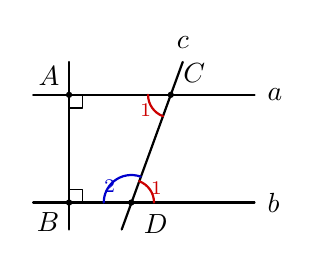
\begin{tikzpicture}[scale=0.76, >=stealth, line join=round, line cap=round]
  % Duong thang a va b
  \draw[thick] (0.2, 2.30) -- (3.9, 2.30) node[right=1pt] {$a$};
  \draw[thick] (0.2, 0.50) -- (3.9, 0.50) node[right=1pt] {$b$};
  
  % Doan thang vuong goc AB
  \draw[thick] (0.80, 0.05) -- (0.80, 2.85);
  \fill (0.80, 2.30) circle (1.5pt) node[above left] {$A$};
  \fill (0.80, 0.50) circle (1.5pt) node[below left] {$B$};
  
  % Ki hieu goc vuong tai A va B
  \draw (0.80, 2.08) -- (1.02, 2.08) -- (1.02, 2.30);
  \draw (0.80, 0.72) -- (1.02, 0.72) -- (1.02, 0.50);
  
  % Cat tuyen c (ve tu bot den top de node c o tren cung)
  \draw[thick] (1.68, 0.05) -- (2.70, 2.85) node[above=1pt] {$c$};
  \fill (2.50, 2.30) circle (1.5pt) node[above right=1pt] {$C$};
  \fill (1.84, 0.50) circle (1.5pt) node[below right=1pt] {$D$};
  
  % Cung goc C1 (goc ACD = alpha)
  \draw[red!80!black, thick] (2.50, 2.30) ++(180:0.38) arc (180:250:0.38);
  \node[red!80!black, font=\scriptsize] at (2.08, 2.04) {$1$};
  
  % Cung goc D1 (so le trong voi C1: goc giua Db phai va DC)
  \draw[red!80!black, thick] (1.84, 0.50) ++(0:0.38) arc (0:70:0.38);
  \node[red!80!black, font=\scriptsize] at (2.26, 0.74) {$1$};
  
  % Cung goc D2 (trong cung phia voi C1: goc BDC)
  \draw[blue!80!black, thick] (1.84, 0.50) ++(70:0.46) arc (70:180:0.46);
  \node[blue!80!black, font=\scriptsize] at (1.48, 0.78) {$2$};
\end{tikzpicture}
\end{minipage}\par
\vspace{0.4mm}
\noindent\textit{Bài giải:}\dongke{11}
\\ \hline
\end{tabularx}

\vspace{1.2mm}

\noindent
\begin{tabularx}{\linewidth}{|X|}
\hline
\vspace{0.5mm}
\textbf{Câu 14 (1,0 điểm).} Cho biểu thức $A = \frac{1}{2} + \frac{1}{2^2} + \frac{1}{2^3} + \dots + \frac{1}{2^{100}}$. Chứng minh rằng $A < 1$.\par
\vspace{0.4mm}
\noindent\textit{Bài giải:}\dongke{8}
\\ \hline
\end{tabularx}

\newpage
% =============================================================================
% ========================= TOÁN 7 - TUẦN 07 - BUỔI 02: MÃ ĐỀ 102 =============
% ========================= MẶT TRƯỚC (TRANG 1/2) ==============================
% =============================================================================

\noindent
\begin{tabularx}{\linewidth}{|X|c|}
\hline
\textbf{PHIẾU KIỂM TRA ĐỊNH KỲ TOÁN 7 - TUẦN 07 - BUỔI 02} & \textbf{Mã đề: 102 - Trang 1/2} \\
\hline
\end{tabularx}

\vspace{1.2mm}

\noindent
\begin{tabularx}{\linewidth}{|p{3.2cm}|X|}
\hline
\centering\textbf{ĐIỂM SỐ} & \centering\textbf{LỜI NHẬN XÉT CỦA THẦY CÔ} \tabularnewline
\hline
\rule{0pt}{1.8cm} & \tabularnewline
\hline
\end{tabularx}

\vspace{1.2mm}

\noindent\textbf{Câu 1 (0,25 điểm).} Trong định lí: \textit{"Nếu hai đường thẳng phân biệt cùng song song với một đường thẳng thứ ba thì chúng song song với nhau"}, phần kết luận là gì? \shortans{chúng song song với nhau}\par\vspace{0.35mm}
\noindent\textbf{Câu 2 (0,25 điểm).} Giá trị của biểu thức $\sqrt{144} - \sqrt{49}$ bằng bao nhiêu? \shortans{5}\par\vspace{0.35mm}
\noindent\textbf{Câu 3 (0,25 điểm).} Giá trị của biểu thức $\vert -5{,}6\vert + \vert 3{,}4\vert$ bằng bao nhiêu? \shortans{9}\par\vspace{0.35mm}
\noindent\textbf{Câu 4 (0,25 điểm).} Làm tròn số $28{,}374$ đến hàng phần mười (chữ số thập phân thứ nhất). \shortans{28{,}4}\par\vspace{0.35mm}
\noindent\textbf{Câu 5 (0,25 điểm).} Cho hai góc $\widehat{xOy}$ và $\widehat{yOz}$ kề bù, biết $\widehat{xOy} = 70^\circ$. Số đo góc $\widehat{yOz}$ là: \shortans{110^\circ}\par\vspace{0.35mm}
\noindent\textbf{Câu 6 (0,25 điểm).} Cho $a \parallel b$ và $c \perp a$. Quan hệ giữa đường thẳng $c$ và đường thẳng $b$ là: \shortans{vuông góc}\par\vspace{0.35mm}
\noindent\textbf{Câu 7 (0,25 điểm).} Giá trị của biểu thức $\left(-\frac{3}{4}\right)^2 + \frac{7}{16}$ bằng bao nhiêu? \shortans{1}\par\vspace{0.35mm}
\noindent\textbf{Câu 8 (0,25 điểm).} Cho tia $Oz$ là tia phân giác của $\widehat{xOy} = 76^\circ$. Số đo góc $\widehat{xOz}$ là: \shortans{38^\circ}\par\vspace{0.35mm}
\noindent\textbf{Câu 9 (0,25 điểm).} Tìm số thực $x \ge 0$, biết $\sqrt{x} = 7$. \shortans{49}\par\vspace{0.35mm}
\noindent\textbf{Câu 10 (0,25 điểm).} Cuốn từ điển giá $150\,000$ đ được giảm $20\%$. Số tiền được giảm là: \shortans{30\,000\text{ đ}}\par\vspace{0.35mm}
\vspace{0.6mm}

\noindent\textbf{Câu 11 (2,0 điểm). Thực hiện phép tính (hợp lý nếu có thể):}
\vspace{0.6mm}

\noindent
\begin{tabularx}{\linewidth}{|X|X|}
\hline
\oBaiTap[8]{a)}{$\frac{5}{18} + \left(-\frac{7}{4}\right) + \frac{13}{18}$} & 
\oBaiTap[8]{b)}{$\frac{4}{11} \cdot \left(-\frac{9}{17}\right) + \frac{4}{11} \cdot \left(-\frac{8}{17}\right)$} \\
\hline
\oBaiTap[8]{c)}{$\left(-\frac{1}{3}\right)^2 \cdot 27 - 2{,}5 \cdot 4$} & 
\oBaiTap[8]{d)}{$\sqrt{\frac{64}{25}} - \vert -0{,}6\vert + \sqrt{100}$} \\
\hline
\end{tabularx}

\newpage
% =============================================================================
% ========================= TOÁN 7 - TUẦN 07 - BUỔI 02: MÃ ĐỀ 102 =============
% ========================= MẶT SAU (TRANG 2/2) ================================
% =============================================================================

\noindent
\begin{tabularx}{\linewidth}{|X|c|}
\hline
\textbf{TOÁN 7 - TUẦN 07 - BUỔI 02} & \textbf{Mã đề: 102 - Trang 2/2} \\
\hline
\end{tabularx}

\vspace{1.2mm}

\noindent\textbf{Câu 12 (2,0 điểm). Tìm số hữu tỉ $x$, biết:}
\vspace{0.6mm}

\noindent
\begin{tabularx}{\linewidth}{|X|X|}
\hline
\oBaiTap[5]{a)}{$x - \frac{1}{4} = \frac{7}{16}$} & 
\oBaiTap[5]{b)}{$\frac{3}{4}x + \frac{1}{5} = \frac{19}{20}$} \\
\hline
\oBaiTap[5]{c)}{$\left(x + \frac{1}{3}\right)^2 = \frac{25}{36}$} & 
\oBaiTap[5]{d)}{$\vert 2x + 3\vert = 9$} \\
\hline
\end{tabularx}

\vspace{1.2mm}

\noindent
\begin{tabularx}{\linewidth}{|X|}
\hline
\vspace{0.5mm}
\begin{minipage}[t]{0.67\linewidth}
\vspace{0pt}
\textbf{Câu 13 (2,5 điểm).} Cho hình vẽ bên, biết đường thẳng $a \perp AB$ tại $A$ và $b \perp AB$ tại $B$. Đường thẳng $c$ cắt $a$ tại $C$ và cắt $b$ tại $D$ tạo thành góc $\widehat{C}_1 = 65^\circ$.\par\vspace{0.4mm}
\textbf{a) (1,25 điểm)} Ghi Giả thiết (GT), Kết luận (KL) của bài toán. Chứng minh rằng $a \parallel b$.\par\vspace{0.4mm}
\textbf{b) (1,25 điểm)} Hãy tính số đo của góc so le trong $\widehat{D}_1$ và góc trong cùng phía $\widehat{D}_2$ với góc $\widehat{C}_1$.
\end{minipage}\hfill
\begin{minipage}[t]{0.31\linewidth}
\vspace{0pt}\centering
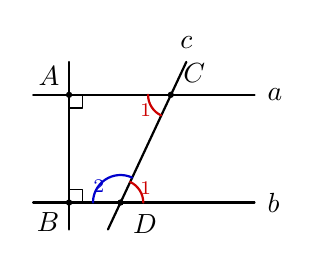
\begin{tikzpicture}[scale=0.76, >=stealth, line join=round, line cap=round]
  % Duong thang a va b
  \draw[thick] (0.2, 2.30) -- (3.9, 2.30) node[right=1pt] {$a$};
  \draw[thick] (0.2, 0.50) -- (3.9, 0.50) node[right=1pt] {$b$};
  
  % Doan thang vuong goc AB
  \draw[thick] (0.80, 0.05) -- (0.80, 2.85);
  \fill (0.80, 2.30) circle (1.5pt) node[above left] {$A$};
  \fill (0.80, 0.50) circle (1.5pt) node[below left] {$B$};
  
  % Ki hieu goc vuong tai A va B
  \draw (0.80, 2.08) -- (1.02, 2.08) -- (1.02, 2.30);
  \draw (0.80, 0.72) -- (1.02, 0.72) -- (1.02, 0.50);
  
  % Cat tuyen c (ve tu bot den top de node c o tren cung)
  \draw[thick] (1.45, 0.05) -- (2.76, 2.85) node[above=1pt] {$c$};
  \fill (2.50, 2.30) circle (1.5pt) node[above right=1pt] {$C$};
  \fill (1.66, 0.50) circle (1.5pt) node[below right=1pt] {$D$};
  
  % Cung goc C1 (goc ACD = alpha)
  \draw[red!80!black, thick] (2.50, 2.30) ++(180:0.38) arc (180:245:0.38);
  \node[red!80!black, font=\scriptsize] at (2.08, 2.04) {$1$};
  
  % Cung goc D1 (so le trong voi C1: goc giua Db phai va DC)
  \draw[red!80!black, thick] (1.66, 0.50) ++(0:0.38) arc (0:65:0.38);
  \node[red!80!black, font=\scriptsize] at (2.08, 0.74) {$1$};
  
  % Cung goc D2 (trong cung phia voi C1: goc BDC)
  \draw[blue!80!black, thick] (1.66, 0.50) ++(65:0.46) arc (65:180:0.46);
  \node[blue!80!black, font=\scriptsize] at (1.30, 0.78) {$2$};
\end{tikzpicture}
\end{minipage}\par
\vspace{0.4mm}
\noindent\textit{Bài giải:}\dongke{11}
\\ \hline
\end{tabularx}

\vspace{1.2mm}

\noindent
\begin{tabularx}{\linewidth}{|X|}
\hline
\vspace{0.5mm}
\textbf{Câu 14 (1,0 điểm).} Cho biểu thức $B = \frac{1}{3} + \frac{1}{3^2} + \frac{1}{3^3} + \dots + \frac{1}{3^{100}}$. Chứng minh rằng $B < \frac{1}{2}$.\par
\vspace{0.4mm}
\noindent\textit{Bài giải:}\dongke{8}
\\ \hline
\end{tabularx}

\newpage
% =============================================================================
% ========================= TOÁN 7 - TUẦN 07 - BUỔI 02: MÃ ĐỀ 103 =============
% ========================= MẶT TRƯỚC (TRANG 1/2) ==============================
% =============================================================================

\noindent
\begin{tabularx}{\linewidth}{|X|c|}
\hline
\textbf{PHIẾU KIỂM TRA ĐỊNH KỲ TOÁN 7 - TUẦN 07 - BUỔI 02} & \textbf{Mã đề: 103 - Trang 1/2} \\
\hline
\end{tabularx}

\vspace{1.2mm}

\noindent
\begin{tabularx}{\linewidth}{|p{3.2cm}|X|}
\hline
\centering\textbf{ĐIỂM SỐ} & \centering\textbf{LỜI NHẬN XÉT CỦA THẦY CÔ} \tabularnewline
\hline
\rule{0pt}{1.8cm} & \tabularnewline
\hline
\end{tabularx}

\vspace{1.2mm}

\noindent\textbf{Câu 1 (0,25 điểm).} Trong định lí: \textit{"Nếu hai đường thẳng phân biệt cùng vuông góc với một đường thẳng thứ ba thì chúng song song với nhau"}, phần kết luận là gì? \shortans{chúng song song với nhau}\par\vspace{0.35mm}
\noindent\textbf{Câu 2 (0,25 điểm).} Giá trị của biểu thức $\sqrt{169} - \sqrt{64}$ bằng bao nhiêu? \shortans{5}\par\vspace{0.35mm}
\noindent\textbf{Câu 3 (0,25 điểm).} Giá trị của biểu thức $\vert -6{,}8\vert + \vert 3{,}2\vert$ bằng bao nhiêu? \shortans{10}\par\vspace{0.35mm}
\noindent\textbf{Câu 4 (0,25 điểm).} Làm tròn số $35{,}628$ đến hàng phần mười (chữ số thập phân thứ nhất). \shortans{35{,}6}\par\vspace{0.35mm}
\noindent\textbf{Câu 5 (0,25 điểm).} Cho hai góc $\widehat{xOy}$ và $\widehat{yOz}$ kề bù, biết $\widehat{xOy} = 80^\circ$. Số đo góc $\widehat{yOz}$ là: \shortans{100^\circ}\par\vspace{0.35mm}
\noindent\textbf{Câu 6 (0,25 điểm).} Cho $a \parallel b$ và $b \parallel c$. Quan hệ giữa hai đường thẳng phân biệt $a$ và $c$ là: \shortans{song song}\par\vspace{0.35mm}
\noindent\textbf{Câu 7 (0,25 điểm).} Giá trị của biểu thức $\left(-\frac{4}{5}\right)^2 + \frac{9}{25}$ bằng bao nhiêu? \shortans{1}\par\vspace{0.35mm}
\noindent\textbf{Câu 8 (0,25 điểm).} Cho tia $Oz$ là tia phân giác của $\widehat{xOy} = 92^\circ$. Số đo góc $\widehat{xOz}$ là: \shortans{46^\circ}\par\vspace{0.35mm}
\noindent\textbf{Câu 9 (0,25 điểm).} Tìm số thực $x \ge 0$, biết $\sqrt{x} = 6$. \shortans{36}\par\vspace{0.35mm}
\noindent\textbf{Câu 10 (0,25 điểm).} Bộ đồng phục giá $250\,000$ đ được giảm $20\%$. Số tiền được giảm là: \shortans{50\,000\text{ đ}}\par\vspace{0.35mm}
\vspace{0.6mm}

\noindent\textbf{Câu 11 (2,0 điểm). Thực hiện phép tính (hợp lý nếu có thể):}
\vspace{0.6mm}

\noindent
\begin{tabularx}{\linewidth}{|X|X|}
\hline
\oBaiTap[8]{a)}{$\frac{8}{21} + \left(-\frac{5}{3}\right) + \frac{13}{21}$} & 
\oBaiTap[8]{b)}{$\frac{6}{13} \cdot \left(-\frac{11}{19}\right) + \frac{6}{13} \cdot \left(-\frac{8}{19}\right)$} \\
\hline
\oBaiTap[8]{c)}{$\left(-\frac{1}{2}\right)^3 \cdot 32 + 2{,}5 \cdot (-4)$} & 
\oBaiTap[8]{d)}{$\sqrt{\frac{81}{16}} - \vert -1{,}25\vert + \sqrt{64}$} \\
\hline
\end{tabularx}

\newpage
% =============================================================================
% ========================= TOÁN 7 - TUẦN 07 - BUỔI 02: MÃ ĐỀ 103 =============
% ========================= MẶT SAU (TRANG 2/2) ================================
% =============================================================================

\noindent
\begin{tabularx}{\linewidth}{|X|c|}
\hline
\textbf{TOÁN 7 - TUẦN 07 - BUỔI 02} & \textbf{Mã đề: 103 - Trang 2/2} \\
\hline
\end{tabularx}

\vspace{1.2mm}

\noindent\textbf{Câu 12 (2,0 điểm). Tìm số hữu tỉ $x$, biết:}
\vspace{0.6mm}

\noindent
\begin{tabularx}{\linewidth}{|X|X|}
\hline
\oBaiTap[5]{a)}{$x - \frac{1}{5} = \frac{9}{25}$} & 
\oBaiTap[5]{b)}{$\frac{4}{5}x - \frac{1}{2} = \frac{3}{10}$} \\
\hline
\oBaiTap[5]{c)}{$\left(x - \frac{1}{4}\right)^2 = \frac{49}{64}$} & 
\oBaiTap[5]{d)}{$\vert 3x - 2\vert = 7$} \\
\hline
\end{tabularx}

\vspace{1.2mm}

\noindent
\begin{tabularx}{\linewidth}{|X|}
\hline
\vspace{0.5mm}
\begin{minipage}[t]{0.67\linewidth}
\vspace{0pt}
\textbf{Câu 13 (2,5 điểm).} Cho hình vẽ bên, biết đường thẳng $a \perp AB$ tại $A$ và $b \perp AB$ tại $B$. Đường thẳng $c$ cắt $a$ tại $C$ và cắt $b$ tại $D$ tạo thành góc $\widehat{C}_1 = 75^\circ$.\par\vspace{0.4mm}
\textbf{a) (1,25 điểm)} Ghi Giả thiết (GT), Kết luận (KL) của bài toán. Chứng minh rằng $a \parallel b$.\par\vspace{0.4mm}
\textbf{b) (1,25 điểm)} Hãy tính số đo của góc so le trong $\widehat{D}_1$ và góc trong cùng phía $\widehat{D}_2$ với góc $\widehat{C}_1$.
\end{minipage}\hfill
\begin{minipage}[t]{0.31\linewidth}
\vspace{0pt}\centering
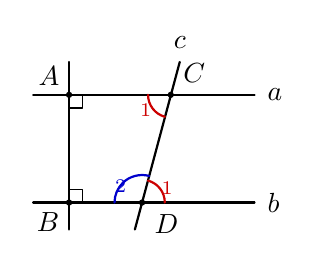
\begin{tikzpicture}[scale=0.76, >=stealth, line join=round, line cap=round]
  % Duong thang a va b
  \draw[thick] (0.2, 2.30) -- (3.9, 2.30) node[right=1pt] {$a$};
  \draw[thick] (0.2, 0.50) -- (3.9, 0.50) node[right=1pt] {$b$};
  
  % Doan thang vuong goc AB
  \draw[thick] (0.80, 0.05) -- (0.80, 2.85);
  \fill (0.80, 2.30) circle (1.5pt) node[above left] {$A$};
  \fill (0.80, 0.50) circle (1.5pt) node[below left] {$B$};
  
  % Ki hieu goc vuong tai A va B
  \draw (0.80, 2.08) -- (1.02, 2.08) -- (1.02, 2.30);
  \draw (0.80, 0.72) -- (1.02, 0.72) -- (1.02, 0.50);
  
  % Cat tuyen c (ve tu bot den top de node c o tren cung)
  \draw[thick] (1.90, 0.05) -- (2.65, 2.85) node[above=1pt] {$c$};
  \fill (2.50, 2.30) circle (1.5pt) node[above right=1pt] {$C$};
  \fill (2.02, 0.50) circle (1.5pt) node[below right=1pt] {$D$};
  
  % Cung goc C1 (goc ACD = alpha)
  \draw[red!80!black, thick] (2.50, 2.30) ++(180:0.38) arc (180:255:0.38);
  \node[red!80!black, font=\scriptsize] at (2.08, 2.04) {$1$};
  
  % Cung goc D1 (so le trong voi C1: goc giua Db phai va DC)
  \draw[red!80!black, thick] (2.02, 0.50) ++(0:0.38) arc (0:75:0.38);
  \node[red!80!black, font=\scriptsize] at (2.44, 0.74) {$1$};
  
  % Cung goc D2 (trong cung phia voi C1: goc BDC)
  \draw[blue!80!black, thick] (2.02, 0.50) ++(75:0.46) arc (75:180:0.46);
  \node[blue!80!black, font=\scriptsize] at (1.66, 0.78) {$2$};
\end{tikzpicture}
\end{minipage}\par
\vspace{0.4mm}
\noindent\textit{Bài giải:}\dongke{11}
\\ \hline
\end{tabularx}

\vspace{1.2mm}

\noindent
\begin{tabularx}{\linewidth}{|X|}
\hline
\vspace{0.5mm}
\textbf{Câu 14 (1,0 điểm).} Cho biểu thức $C = \frac{1}{4} + \frac{1}{4^2} + \frac{1}{4^3} + \dots + \frac{1}{4^{100}}$. Chứng minh rằng $C < \frac{1}{3}$.\par
\vspace{0.4mm}
\noindent\textit{Bài giải:}\dongke{8}
\\ \hline
\end{tabularx}

\newpage
% =============================================================================
% ========================= TOÁN 7 - TUẦN 07 - BUỔI 02: MÃ ĐỀ 104 =============
% ========================= MẶT TRƯỚC (TRANG 1/2) ==============================
% =============================================================================

\noindent
\begin{tabularx}{\linewidth}{|X|c|}
\hline
\textbf{PHIẾU KIỂM TRA ĐỊNH KỲ TOÁN 7 - TUẦN 07 - BUỔI 02} & \textbf{Mã đề: 104 - Trang 1/2} \\
\hline
\end{tabularx}

\vspace{1.2mm}

\noindent
\begin{tabularx}{\linewidth}{|p{3.2cm}|X|}
\hline
\centering\textbf{ĐIỂM SỐ} & \centering\textbf{LỜI NHẬN XÉT CỦA THẦY CÔ} \tabularnewline
\hline
\rule{0pt}{1.8cm} & \tabularnewline
\hline
\end{tabularx}

\vspace{1.2mm}

\noindent\textbf{Câu 1 (0,25 điểm).} Trong định lí: \textit{"Nếu hai góc đối đỉnh thì hai góc đó bằng nhau"}, phần kết luận là gì? \shortans{hai góc đó bằng nhau}\par\vspace{0.35mm}
\noindent\textbf{Câu 2 (0,25 điểm).} Giá trị của biểu thức $\sqrt{196} - \sqrt{81}$ bằng bao nhiêu? \shortans{5}\par\vspace{0.35mm}
\noindent\textbf{Câu 3 (0,25 điểm).} Giá trị của biểu thức $\vert -7{,}5\vert + \vert 4{,}5\vert$ bằng bao nhiêu? \shortans{12}\par\vspace{0.35mm}
\noindent\textbf{Câu 4 (0,25 điểm).} Làm tròn số $42{,}865$ đến hàng phần mười (chữ số thập phân thứ nhất). \shortans{42{,}9}\par\vspace{0.35mm}
\noindent\textbf{Câu 5 (0,25 điểm).} Cho hai góc $\widehat{xOy}$ và $\widehat{yOz}$ kề bù, biết $\widehat{xOy} = 50^\circ$. Số đo góc $\widehat{yOz}$ là: \shortans{130^\circ}\par\vspace{0.35mm}
\noindent\textbf{Câu 6 (0,25 điểm).} Hai đường thẳng $xx', yy'$ cắt nhau tại $O$. Nếu $\widehat{xOy} = 90^\circ$ thì góc đối đỉnh $\widehat{x'Oy'}$ bằng: \shortans{90^\circ}\par\vspace{0.35mm}
\noindent\textbf{Câu 7 (0,25 điểm).} Giá trị của biểu thức $\left(-\frac{5}{6}\right)^2 + \frac{11}{36}$ bằng bao nhiêu? \shortans{1}\par\vspace{0.35mm}
\noindent\textbf{Câu 8 (0,25 điểm).} Cho tia $Oz$ là tia phân giác của $\widehat{xOy} = 104^\circ$. Số đo góc $\widehat{xOz}$ là: \shortans{52^\circ}\par\vspace{0.35mm}
\noindent\textbf{Câu 9 (0,25 điểm).} Tìm số thực $x \ge 0$, biết $\sqrt{x} = 5$. \shortans{25}\par\vspace{0.35mm}
\noindent\textbf{Câu 10 (0,25 điểm).} Chiếc cặp sách giá $200\,000$ đ giảm $20\%$. Số tiền được giảm là: \shortans{40\,000\text{ đ}}\par\vspace{0.35mm}
\vspace{0.6mm}

\noindent\textbf{Câu 11 (2,0 điểm). Thực hiện phép tính (hợp lý nếu có thể):}
\vspace{0.6mm}

\noindent
\begin{tabularx}{\linewidth}{|X|X|}
\hline
\oBaiTap[8]{a)}{$\frac{7}{20} + \left(-\frac{9}{5}\right) + \frac{13}{20}$} & 
\oBaiTap[8]{b)}{$\frac{7}{15} \cdot \left(-\frac{14}{23}\right) + \frac{7}{15} \cdot \left(-\frac{9}{23}\right)$} \\
\hline
\oBaiTap[8]{c)}{$\left(-\frac{2}{3}\right)^2 \cdot 18 - 3{,}5 \cdot 4$} & 
\oBaiTap[8]{d)}{$\sqrt{\frac{121}{25}} - \vert -1{,}2\vert + \sqrt{49}$} \\
\hline
\end{tabularx}

\newpage
% =============================================================================
% ========================= TOÁN 7 - TUẦN 07 - BUỔI 02: MÃ ĐỀ 104 =============
% ========================= MẶT SAU (TRANG 2/2) ================================
% =============================================================================

\noindent
\begin{tabularx}{\linewidth}{|X|c|}
\hline
\textbf{TOÁN 7 - TUẦN 07 - BUỔI 02} & \textbf{Mã đề: 104 - Trang 2/2} \\
\hline
\end{tabularx}

\vspace{1.2mm}

\noindent\textbf{Câu 12 (2,0 điểm). Tìm số hữu tỉ $x$, biết:}
\vspace{0.6mm}

\noindent
\begin{tabularx}{\linewidth}{|X|X|}
\hline
\oBaiTap[5]{a)}{$x - \frac{1}{6} = \frac{11}{36}$} & 
\oBaiTap[5]{b)}{$\frac{5}{6}x - \frac{1}{3} = \frac{1}{2}$} \\
\hline
\oBaiTap[5]{c)}{$\left(x + \frac{1}{5}\right)^2 = \frac{36}{25}$} & 
\oBaiTap[5]{d)}{$\vert 3x + 4\vert = 10$} \\
\hline
\end{tabularx}

\vspace{1.2mm}

\noindent
\begin{tabularx}{\linewidth}{|X|}
\hline
\vspace{0.5mm}
\begin{minipage}[t]{0.67\linewidth}
\vspace{0pt}
\textbf{Câu 13 (2,5 điểm).} Cho hình vẽ bên, biết đường thẳng $a \perp AB$ tại $A$ và $b \perp AB$ tại $B$. Đường thẳng $c$ cắt $a$ tại $C$ và cắt $b$ tại $D$ tạo thành góc $\widehat{C}_1 = 55^\circ$.\par\vspace{0.4mm}
\textbf{a) (1,25 điểm)} Ghi Giả thiết (GT), Kết luận (KL) của bài toán. Chứng minh rằng $a \parallel b$.\par\vspace{0.4mm}
\textbf{b) (1,25 điểm)} Hãy tính số đo của góc so le trong $\widehat{D}_1$ và góc trong cùng phía $\widehat{D}_2$ với góc $\widehat{C}_1$.
\end{minipage}\hfill
\begin{minipage}[t]{0.31\linewidth}
\vspace{0pt}\centering
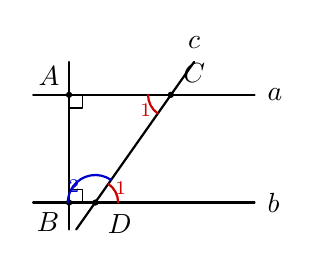
\begin{tikzpicture}[scale=0.76, >=stealth, line join=round, line cap=round]
  % Duong thang a va b
  \draw[thick] (0.2, 2.30) -- (3.9, 2.30) node[right=1pt] {$a$};
  \draw[thick] (0.2, 0.50) -- (3.9, 0.50) node[right=1pt] {$b$};
  
  % Doan thang vuong goc AB
  \draw[thick] (0.80, 0.05) -- (0.80, 2.85);
  \fill (0.80, 2.30) circle (1.5pt) node[above left] {$A$};
  \fill (0.80, 0.50) circle (1.5pt) node[below left] {$B$};
  
  % Ki hieu goc vuong tai A va B
  \draw (0.80, 2.08) -- (1.02, 2.08) -- (1.02, 2.30);
  \draw (0.80, 0.72) -- (1.02, 0.72) -- (1.02, 0.50);
  
  % Cat tuyen c (ve tu bot den top de node c o tren cung)
  \draw[thick] (0.92, 0.05) -- (2.89, 2.85) node[above=1pt] {$c$};
  \fill (2.50, 2.30) circle (1.5pt) node[above right=1pt] {$C$};
  \fill (1.24, 0.50) circle (1.5pt) node[below right=1pt] {$D$};
  
  % Cung goc C1 (goc ACD = alpha)
  \draw[red!80!black, thick] (2.50, 2.30) ++(180:0.38) arc (180:235:0.38);
  \node[red!80!black, font=\scriptsize] at (2.08, 2.04) {$1$};
  
  % Cung goc D1 (so le trong voi C1: goc giua Db phai va DC)
  \draw[red!80!black, thick] (1.24, 0.50) ++(0:0.38) arc (0:55:0.38);
  \node[red!80!black, font=\scriptsize] at (1.66, 0.74) {$1$};
  
  % Cung goc D2 (trong cung phia voi C1: goc BDC)
  \draw[blue!80!black, thick] (1.24, 0.50) ++(55:0.46) arc (55:180:0.46);
  \node[blue!80!black, font=\scriptsize] at (0.88, 0.78) {$2$};
\end{tikzpicture}
\end{minipage}\par
\vspace{0.4mm}
\noindent\textit{Bài giải:}\dongke{11}
\\ \hline
\end{tabularx}

\vspace{1.2mm}

\noindent
\begin{tabularx}{\linewidth}{|X|}
\hline
\vspace{0.5mm}
\textbf{Câu 14 (1,0 điểm).} Cho biểu thức $D = \frac{1}{5} + \frac{1}{5^2} + \frac{1}{5^3} + \dots + \frac{1}{5^{100}}$. Chứng minh rằng $D < \frac{1}{4}$.\par
\vspace{0.4mm}
\noindent\textit{Bài giải:}\dongke{8}
\\ \hline
\end{tabularx}

\newpage
\end{document}